%%%%%%%%%%%%%%%%%%%%%%%%%%%%%%%%%%%%%%%%%%%%%%%%%%%%%%%%%%%%%%%%%%%%%%%%%%%%%%%%%%%%%%%%%%%%%%%%%%%%%
% This template is distributed with ABSOLUTELY NO WARRANTY.
% It serves as a guideline and constitutes a basic structure for a
% thesis/dissertation. The user assumes full responsibility for formatting
% and typesetting their document and for verifying that all the thesis
% requirements set by the University of Tennessee are met. Please refer to the most
% recent UT thesis guide (http://gradschool.utk.edu/thesesdissertations/formatting/)
% or contact the thesis consultant (http://gradschool.utk.edu/thesesdissertations/).
% Please report any bugs to the thesis consultant.
%%%%%%%%%%%%%%%%%%%%%%%%%%%%%%%%%%%%%%%%%%%%%%%%%%%%%%%%%%%%%%%%%%%%%%%%%%%%%%%%%%%%%%%%%%%%%%%%%%%%%
% O P T I O N S:
% 1. thesis/dissertation
% 2. monochrome
% 3. all options provided by the report class
%%%%%%%%%%%%%%%%%%%%%%%%%%%%%%%%%%%%%%%%%%%%%%%%%%%%%%%%%%%%%%%%%%%%%%%%%%%%%%%%%%%%%%%%%%%%%%%%%%%%%
%First, is this a thesis or dissertation? Choose one by commenting out the one you don't need:
%\documentclass[thesis,letterpaper,12pt]{utthesis} % thesis
\documentclass[dissertation,letterpaper,12pt]{utthesis} %dissertation
% some alternatives are:
%\documentclass[thesis,monochrome,letterpaper,12pt]{utthesis} %thesis, monochrome text
\renewcommand{\baselinestretch}{1.5} 	 % line Spacing
%%%%%%%%%%%%%%%%%%%%%%%%%%%%%%%%%%%%%%%%%%%%%%%%%%%%%%%%%%%%%%%%%%%%%%%%%%%%%%%%%%%%%%%%%%%%%%%%%%%%%
% TO DO: FILL IN YOUR INFORMATION BELOW - READ THIS SECTION CAREFULLY
%%%%%%%%%%%%%%%%%%%%%%%%%%%%%%%%%%%%%%%%%%%%%%%%%%%%%%%%%%%%%%%%%%%%%%%%%%%%%%%%%%%%%%%%%%%%%%%%%%%%%
\title{Ontological Considerations for Interoperability in Scientific Workflows}	       	% title of thesis/dissertation
\author{Jay Jay Billings}                			% author's name
\copyrightYear{2019}            				% copyright year of your thesis/dissertation
\graduationMonth{December}           				% month of graduation for your
% thesis/dissertation
\degree{Doctor of Philosophy}	    			% degree: Doctor of Philosophy, Master of Science, Master of Engineering...
\university{The University  of Tennessee, Knoxville}	% school name
%%%%%%%%%%%%%%%%%%%%%%%%%%%%%%%%%%%%%%%%%%%%%%%%%%%%%%%%%%%%%%%%%%%%%%%%%%%%%%%%%%%%%%%%%%%%%%%%%%%%%
% LOAD SOME USEFUL PACKAGES. 
% No need to change anything here, although if you'd like to add packages you
% can do that here. Note that packages preloaded with the utthesis class are:
% amsmath,amsthm,amssymb,setspace,geometry,hyperref,and color
%%%%%%%%%%%%%%%%%%%%%%%%%%%%%%%%%%%%%%%%%%%%%%%%%%%%%%%%%%%%%%%%%%%%%%%%%%%%%%%%%%%%%%%%%%%%%%%%%%%%%
\usepackage{nomencl}                    % produces a nomenclature
\usepackage{float}                      % figure floats
\usepackage[numbers]{natbib}                     % this package allows you to link your references
\usepackage{graphicx}					% graphics package
\graphicspath{ {figures/}{figures/eps/}{figures/pdf/} }% specify the path where figures are located
\usepackage{fancyhdr}                   % fancy headers and footers
\usepackage{url}                        % nicely format url breaks
\usepackage[inactive]{srcltx}		 	% necessary to use forward and inverse searching in DVI
\usepackage{relsize}                    % font sizing hierarchy
\usepackage{booktabs}                   % professional looking tables
\usepackage[config, labelfont={bf}]{caption,subfig} % nice sub figures
\usepackage{mathrsfs}                   % additional math scripts
\usepackage[titletoc]{appendix}			% format appendix correctly
\usepackage{pdflscape}					% to produce landscape pages if necessary
\usepackage{thesistools}				% my thesis tools package for cramming all these papers together
\usepackage{tabularx}					% tabularx package for better tables
\usepackage{todonotes}					% this package captures notes and tasks TO-DO
\usepackage[autostyle]{csquotes} 		% stylish quote package
\usepackage{array}						% array-listing package
\usepackage{tabu}						% alternate table package
\usepackage{listings}					% listings package for code listings, etc.
\usepackage{color}						% Color package for working with the listing package

%%%%%%%%%%%%%%%%%%%%%%%%%%%%%%%%%%%%%%%%%%%%%%%%%%%%%%%%%%%%%%%%%%%%%%%%%%%%%%%%%%%%%%%%%%%%%%%%%%%%%%%
%
% lstlisting settings for syntax highlighting
%
%%%%%%%%%%%%%%%%%%%%%%%%%%%%%%%%%%%%%%%%%%%%%%%%%%%%%%%%%%%%%%%%%%%%%%%%%%%%%%%%%%%%%%%%%%%%%%%%%%%%%%%

% Color definitions
\definecolor{mygreen}{rgb}{0,0.6,0}
\definecolor{mygray}{rgb}{0.5,0.5,0.5}
\definecolor{mymauve}{rgb}{0.58,0,0.82}
\definecolor{maroon}{rgb}{0.5,0,0}
\definecolor{darkgreen}{rgb}{0,0.5,0}

% Basic setup
\lstset{ %
  backgroundcolor=\color{white},   % choose the background color
  basicstyle=\footnotesize,        % size of fonts used for the code
  breaklines=true,                 % automatic line breaking
  breakatwhitespace=false,         % allow breaking in character space
  linewidth=\textwidth,			   % make sure the listings are \textwidth wide
  captionpos=tb,                    % sets the caption-position to top
  commentstyle=\color{mygreen},    % comment style
  escapeinside={\%*}{*)},          % if you want to add LaTeX within your code
  keywordstyle=\color{blue},       % keyword style
  stringstyle=\color{mymauve},     % string literal style
}

% XML redefinition
\lstdefinelanguage{XML} {
  basicstyle=\ttfamily,
  morestring=[s]{"}{"},
  morecomment=[s]{?}{?},
  morecomment=[s]{!--}{--},
  commentstyle=\color{darkgreen},
  moredelim=[s][\color{black}]{>}{<},
  moredelim=[s][\color{red}]{\ }{=},
  stringstyle=\color{blue},
  identifierstyle=\color{maroon}
}

% TURTLE definition
\lstdefinelanguage{TURTL} {
  basicstyle=\ttfamily,
%  morestring=[s]{"}{"},
%  morecomment=[s]{?}{?},
%  morecomment=[s]{\#\#\#}{\\n},
%  commentstyle=\color{darkgreen},
  %moredelim=[s][\color{red}]{@prefi}{x},
  %moredelim=[s][\color{blue}]{rdf}{:},
%  stringstyle=\color{blue},
  identifierstyle=\color{maroon}
}

%%%%%%%%%%%%%%%%%%%%%%%%%%%%%%%%%%%%%%%%%%%%%%%%%%%%%%%%%%%%%%%%%%%%%%%%%%%%%%%%%%%%%%%%%%%%%%%%%%%%%%
% This section formats landscape pages properly with the correct page number.
% This code is only necessary when landscape pages are needed and can be left alone
%%%%%%%%%%%%%%%%%%%%%%%%%%%%%%%%%%%%%%%%%%%%%%%%%%%%%%%%%%%%%%%%%%%%%%%%%%%%%%%%%%%%%%%%%%%%%%%%%%%%%%

\fancypagestyle{mylandscape}{
	\fancyhf{} %Clears the header/footer
	\fancyfoot{% Footer
    \makebox[\textwidth][r]{% Right
      \rlap{\hspace{.75cm}% Push out of margin by \footskip
        \smash{% Remove vertical height
          \raisebox{4.87in}{% Raise vertically
            \rotatebox{90}{\thepage}}}}}}% Rotate counter-clockwise
  \renewcommand{\headrulewidth}{0pt}% No header rule
  \renewcommand{\footrulewidth}{0pt}% No footer rule
}


%%%%%%%%%%%%%%%%%%%%%%%%%%%%%%%%%%%%%%%%%%%%%%%%%%%%%%%%%%%%%%%%%%%%%%%%%%%%%%%%%%%%%%%%%%%%%%%%%%%%%
\begin{document}
    \pagenumbering{alph} % this is needed to clear certain issues with the hyperref package
    %
    \addToPDFBookmarks{0}{Front Matter}{rootNode} % create a root node named "Front Matter" in the pdf bookmarks
    \addToPDFBookmarks{1}{Title}{a} % add a pdf bookmark to the title page
    \makeTitlePage % make the title page.
    %
    \pagenumbering{roman}
    \setcounter{page}{2}
    %
    \makeCopyrightPage % make the copyright page
    %
%%%%%%%%%%%%%%%%%%%%%%%%%%%%%%%%%%%%%%%%%%%%%%%%%%%%%%%%%%%%%%%%%%%%%%%%%%%%%%%%%%%%%%%%%%%%%%%%%%%%%
%The dedication and acknowledgments are optional. If you wish not to include
% them, simply comment out both the "\addToPDF..." line and the "\include{...}" line for each.
%%%%%%%%%%%%%%%%%%%%%%%%%%%%%%%%%%%%%%%%%%%%%%%%%%%%%%%%%%%%%%%%%%%%%%%%%%%%%%%%%%%%%%%%%%%%%%%%%%%%%
    \addToPDFBookmarks{1}{Dedication}{b} % add a pdf bookmark to the dedication page
    \chapter*{}
\begin{center}
{\centering \it dedication... }
\end{center}  % include the dedication

    \addToPDFBookmarks{1}{Acknowledgments}{c} % add a pdf bookmark to the acknowledgments page
    \chapter*{Acknowledgments}

There is an old saying among parents: It takes a village to raise a child. The
same phrase likely applies to the development of any dissertation, and as such
the author would like to acknowledge the contributions and support of the
following fellow villagers.

First, the author's committee requires special acknowledgment and gratitude
for taking on an nontraditional student and an interdisciplinary topic.
Neither are easy and they did both at the same time. The committee includes Jack
Dongarra, John Drake, Mike Guidry (chair), Mallikarjun Shankar, and John Turner. 

The author is grateful for the support provided by the US Department
of Energy and the ORNL Director’s Research and Development Fund in the
Integrated Computational Environment for the Modeling and Analysis of Neutrons
(ICEMAN) project. ORNL is managed by UT-Battelle LLC for the US Department of
Energy under contract DE-AC05-00OR22725. The completion of this work would not
have been possible without the continued encouragement and uplifting support of
colleagues and management at ORNL. The author is also grateful to the management
and staff of RNET Technologies LLC, especially Gerald Sabin and Ben O'Neill, who
supported part of this work under subcontract to ORNL.

The author would like to express his sincere thanks to his coauthors and
fellow developers of the Eclipse Integrated Computational Environment that
forms much of the foundation of this work. These collaborators include Andrew
Bennett, Jordan Deyton, Kasper Gammeltoft, Jonah, Graham, Dasha Gorin, Hari
Krishnan, Menghan Li, Alexander J. McCaskey, Taylor Patterson, Robert Smith,
Gregory Watson, and Anna Wojtowicz. Other collaborators who the author would
like to acknowledge for thoughtful discussions on workflows include Jim Belak on
the nature of workflows in the ExAM project, and Robert Clay, Dan Laney, and
David Montoya on modeling and simulation workflows. The earliest work on this
project included substantial effort by many others who directly or
indirectly contributed to the project, either in its early days as “NiCE” or
once it moved to Eclipse. This includes Ronald Allen, Andrew Belt, David E.
Bernholdt, Tim Bohn, Erica Grant, John M. Hetrick III, Forest Hull, Sebastien
Jourdain, JiSoo Kim, Allison Koenecke, Fangzhou Lin, Eric J. Lingerfelt, Greg
Lyon, Tony McCrary, Elizabeth Piersall, Neeti Pokhriyal, Adrian Sanchez, Claire
Saunders, Nick Stanish, Matthew Wang, ivand Scott Wittenberg. The authors would
like to acknowledge the special contribution of the Eclipse Foundation, the
Eclipse Community, the Eclipse Science Working Group, and our many colleagues
who use and contribute to open-source projects in the Eclipse ecosystem.
Finally, the development team is especially grateful to Barney Maccabe, David
Pointer for their endless support and advocacy for this work.

The author is grateful for the information and citations on Scrybe from Anthony
Skjellum, Director of the SimCenter at the University of Tennessee,
Chattanooga. The author is also grateful to the internal reviewers and helpful
colleagues at the Oak Ridge National Laboratory, and many other anonymous
reviewers who provided feedback on the journal articles and conference
presentations that sprung from this work.

Shantenu Jha of Rutgers and Brookhaven National Laboratory, and Katie Knight, of
Oak Ridge National Laboratory, deserve their own acknowledgements chapter and
together could easily serve as the model for an entire ontology for ``Ideal
Colleagues.'' The kindness, encouragment, and continued support, as well as the
constant willingness to act as a sounding board for crazy ideas has earned these
perpetual thanks and beer at the authors expense.

Charlie Horak edited this work, including the author's bad references to Star
Trek in Chapter \ref{ch:ontologies}, and the author is grateful for her patience
dealing with inconsistent commas, tense switching, bad numbering, and a number
of other things that are not in the version the reader is holding thanks to her
efforts.

An extremely large amount of peanut butter and chocolate was consumed in the
creation of this work. This includes a very large amount of the Peanut Butter
Fudge ice cream available at the Island Scoop Restaurant in Jamestown Rhode
Island. The author appreciates the kindness of the proprietor(s) and staff who
let him crash at the restaurant for several hours a day while he worked on
corrections during his family vacation.

Last but not least, the author would like to acknowledge the sacrifies made by
and continuous support and love from his wife and daughter, both of whom
constantly encouraged him, even on vacation, to complete this work. Of all the
villagers who made this possible, none did more than these two and the author
expresses his extreme gratitude and love to them.
 % include the acknowledgments
    
    \addToPDFBookmarks{1}{Abstract}{e} % add a pdf bookmark to the abstract page
    \chapter*{Abstract}\label{ch:abstract}

Scientific workflows exist in many different domains and for many different
computing platforms. As these systems have proliferated, they have also become
increasingly complex and harder to maintain. Furthermore, these systems often
exist as self-sufficient islands of capability that can be over-specialized and
locked into a specific domain. Some commonality exists and three major workflow
types are readily apparent in (i) modeling and simulation, (ii) high-throughput
data analysis, and (iii) optimization. A far more detailed understanding of
different workflow types is required to determine how large, interdisciplinary
workflows that span the types and multiple computing facilities can be created
and executed. This work presents a new model of scientific workflows that
attempts to create such an understanding with a formal, machine-readable
ontology that can be used to answer design questions about interoperability for
workflows that need to be executed across distributed workflow management
systems. Example instances are presented for simple workflows that do not
require decision making, more complicated workflows that can split decision
making between external agents and internal state transitions in finite state
machines, and purely conceptual workflows that represent notional if not exactly
executable workflows purely for communicating ideas. Finally, a perspective on
interoperability for workflow systems is presented in the context of the
ontology. % your abstract

    \addToPDFBookmarks{0}{Table of Contents}{f}
    \tableofcontents % generate a table of contents
    \listoftables % generate a list of tables
    \listoffigures % generate a list of figures
   
    \newpage
    \pagenumbering{arabic}
    \setcounter{page}{1}
    %%%%%%%%%%%%%%%%%%%%%%%%%%%%%%%%%%%%%%%%%%%%%%%%%%%%%%%%%%%%%%%%%%%%%%%%%%%%%%%%%%%%%%%%%%%%%%%%%%%%%
    % INCLUDE THE CHAPTERS STARTING WITH THE NOMENCLATURE IF PRESENT
    %%%%%%%%%%%%%%%%%%%%%%%%%%%%%%%%%%%%%%%%%%%%%%%%%%%%%%%%%%%%%%%%%%%%%%%%%%%%%%%%%%%%%%%%%%%%%%%%%%%%%
    \include{front-matter}
    \chapter{Introduction} \label{ch:introduction}
\todo{Need a statement somewhere that more work has gone into systems than
workflows per se.}

Many civilizations tell an origin story for the diversity of human language. The
common thread in different versions of this story is that humanity
originally spoke a single language and united together to build a tower so tall
that it could reach heaven. Some versions say that the builders used blocks of
a common size, while others say that the builders used timbers of a common
length. The end is the same in most versions: When God learns of the
tower, he punishes the builders by confusing them, and then spreads them across
the world. The tower is left unfinished, heaven is left untouched, and the
builders are left speaking different languages.

Through an amount of research effort roughly equally to the work required
to build a sky-high tower, modern linguistics has demonstrated the low
likelihood of an original, single human language. However, the insights gained
about the nature of language, human anatomy, learning and neuroscience from this
effort were very valuable in their own right because of what they enabled or
revealed in other research efforts.

As complex as human language may be, computer science may represent the ultimate
test of our ability to study diverse ecosystems with new languages and tools
under constant, continuous development. Language and tool diversity is a
benefit to computing because each new language or tool is designed purposely to
solve a new problem, or to solve an old problem in a new way. This allows for
the entire technology stack to  be layered, optimized, and deployed in ways
specifically designed to exploit favorable conditions in complex systems. Case
in point, older programming languages such as Fortran and Kobol did not lose
popularity because of divine intervention. They lost popularity because of
economic forces that drove the development and adoption of more portable and
expressive system languages, such as C. Fortran and Kobol are still used in
places where they make sense, including high performance computing and finance,
but better tools are used where Fortran and Kobol are less than optimal.

One important class of programming languages and tools includes those that
can be combined with data to streamline and, in many cases, automate the
execution of tasks and processes. The major advantage of these tools is that
they make previously cumbersome activities repeatable and highly efficient.
This class solves \textit{workflow problems}, and is especially noteworthy
because of the poorly understood panoply of tools found in this space.

This work examines workflow problems and assocciated technology under two
assumptions that can be seen in parallel with broader
computing ecosystem. Specifically it considers that 1) there are no preferred
universal languages or tools, and 2) a lack of standardization
in software solutions is common because it is beneficial. Based
on these assumptions, this work shows that 
\begin{itemize}
  \item the workflow technology space is well covered by different types
  of systems,
  \item that an ontological treatment can be used to create a map of
  workflows and workflow management systems,
  \item and that this map can be used for next generation
  challenges such system interoperability and decision making.
\end{itemize}

The present chapter provides a thorough introduction of the workflow problem
space as well as some philosopical background to prepare the reader. Chapter
\ref{ch:ontologies} discusses ontologies, associated tools, and ontological
models relevant to workflows. Interoperability enabled solely through
ontological considerations is presented in chapter
\ref{ch:interoperability}. Chapter \ref{ch:eclipse-ice} introduces the
Eclipse Integrated Computational Environment (Eclipse ICE), which acted as the
primary model and served as a starting point for much of the
ontological and technical work. Chapter \ref{ch:blockchain} details a new model
data management and provenance capture for scientific workflows that embodies
the principles shared herein. A final summary and discussion of the
value of and opportunities for future work are presented in chapter
\ref{ch:conclusions}.

\subsubsection{Content sources}

The content in this document is largely based on separately published papers
that were collected, expanded, and edited for the purposes of better supporting
the argumentative stance of a thesis, and the formatting requirements of
the graduate school. The introductory text in this chapter is largely based on
work published previously in the Open Source Supercomputing workshop,
\cite{billings_toward_2017}. The content of chapter \ref{ch:eclipse-ice} was
adapted from a manuscript in the journal Software X,
\cite{billings_eclipse_2017}. The data management system in chapter
\ref{ch:blockchain} includes work presented as an invited talk at the First
International Workshop on Practical Reproducible Evaluation of Computer Systems
(P-RECS'18) with additional content on new work and the software system, the
\textit{Basic Artifact Tracking System (BATS)}, which has entered production
use. Additional content has been adapted from slides presented at international
conferences and workshops, as well as committee meetings.

The ontological and classification work presented in chapters
\ref{ch:ontologies} and \ref{ch:interoperability} is completely new, and at
time of this writing has not been published in manuscript form in
workshop, conference, or journal. However, the full source of the ontologies
and code has been made available on Github.com in the Eclipse ICE repository,
\cite{billings_ice}.

\todo{FIX the Eclipse ICE reference needs to be updated to
point to Software X}
\todo{the GitHub Eclipse ICE reference needs to be checked}

\section{Workflows}

\todo{Review CBB section}
\textit{The role that CBBs can play are at a system level. The section can be
reframed based on that.}

\baseInclude{pubs/workflows-paper/src/introduction}
\baseInclude{pubs/workflows-paper/src/workflows-review}
\baseInclude{pubs/workflows-paper/src/experience}
\baseInclude{pubs/workflows-paper/src/common}
\baseInclude{pubs/workflows-paper/src/buildingblocks}

\section{Summary}

The previous sections illustrate the complexity and diversity of workflow
technologies. Having amassed such data on the topic, it is tempting to develop
a new or adopt an existing definition of ``workflow'' and ``workflow system.''
However, settling on a single, simple definition has not worked well in the past
for a wide enough cross section of the community to meet future needs as workflows
begin to integrate experimental, computational, and analytical processes at
larger scales. Even more rigorous methods that attempt to create relevant
taxonomies are restricted to a single community, such as grid workflows in the
case of Yu and Buyya.

It is highly desirable to develop a deeper understanding of the similarities and
differences between workflows and related systems for several reasons. First, if
unnecessary duplication can be avoided and a greater understanding gained, they
should be to help with decision making and resource allocation. Second, a
deeper understanding may make it possible to do new, highly desirable things
with workflow management systems. Finally, it may reveal new ways to improve or
use related technologies including data management, machine learning, and
artificial intelligence.

Ontologies are efficient tools for gaining such an understanding as they
can formally catalog all of the different properties relevant to gaining
knowledge in a given topical area. This can be done in both human and machine
readable ways. The following chapters provide just such an analysis. However,
before turning to ontological considerations, and in an effort to better
understand the origins of the questions at the core of this thesis, it is
important to look at an interesting and somewhat unique workflow management
system: The Eclipse Integrated Computational Environment.


    \chapter{The Eclipse Integrated Computational Environment} \label{ch:eclipse-ice}

The previous chapter described two assumptions about workflow management
systems, namely that 1) there are no preferred universal languages or tools
and 2) a lack of standardization in software solutions is common because it is
beneficial. Further, that chapter also asserts that an ontological approach
could be used to develop a map of workflow management systems. Those assumptions
and the idea of a scientific workflow ontology arose from nearly a decade of
research into the topic as part of the effort to develop workflow tools for
high-performance modeling and simulation applications. One key realization
during this work was that the system under development could aggregate and share
other workflow engines relatively easily and without significant changes to the
code base \cite{brooks_introducing_2016}. This suggested that it was possible
to develop a more general, possibly common understanding of workflows and
workflow management systems. That system, the Eclipse Integrated Computational
Environment, is discussed in detail below to introduce concepts that will be
necessary in the development of a scientific workflow ontology in later
chapters.

\baseInclude{pubs/ice-softwarex-2017/src/content}

\section{Summary}

This chapter presents an overview of Eclipse ICE, including a discussion on its
position within the broader workflow management system ecosystem and its
workflow model. The overall architecture of Eclipse ICE version 2.0 is
described, and several examples are presented to illustrate its applicability
to modeling and simulation problems. Samples and tutorials are also provided
for the eager and interested reader.

\baseInclude{pubs/ice-softwarex-2017/src/conclusions}

The primary challenge with understanding the differences between Eclipse ICE and
these other systems, as well as how they can be integrated, is the lack of a
standard model that can holistically describe multiple types of workflows. The
following chapter starts the process of developing such a model by
describing tools and techniques for creating ontologies that describe the
entities and relationships of complex systems.

    \chapter{Ontologies} \label{ch:ontologies}

A formal system for describing scientific workflows would be valuable for a
variety of reasons. Perhaps most importantly, this includes being able to
determine what types of systems need to be implemented to successfully execute
the workflow. This is fundamentally a question about our ability to model our
workflows thoroughly without building out a fully functional system, which is
common at present. It is not clear that this current model will continue to
scale up efficiently as workflows become more distributed, hierarchical, and
mixed because of the associated increase in complexity. 

One important tool in understanding complex computing systems is an ontology.
An ontology captures knowledge about a system in a formal way. This includes
capturing details about entities, classes of entities, entity properties, and
the relationships among these things. Ontologies are usually recorded in a
graph data structure. The graph can be modified, linked, or merged with other
ontology graphs to create an even greater understanding of a topic.

This chapter introduces ontologies with a focus on how they can be used to
better understand different types of workflows, workflow management systems,
and workflow data models. First, common properties of ontologies are reviewed to
provide a basic understanding of their use. Second, a short example is provided
to illustrate their use in encoding real-world data. This includes an
illustration of why ontologies are sometimes favored over taxonomies. Finally, a
common set of tools for working with ontologies is presented to illustrate how
ontologies are created in formal ways that are machine-readable, and ready for
distribution and use in larger applications.

\section{Features of Ontologies}

Ontologies are commonly described using special ontology languages, such as the
Web Ontology Language (OWL), or modeling languages like the Unified Modeling
Language (UML). There are a number of common features found across these
languages, some of which are useful for the following discussions. 

\subsection{Properties}

Entities in an ontology can have properties that describe their makeup. Some
entities, such as primitive double precision floating point numbers, have their
value as their only property. However, other entities, such as computers, may
have many properties, including hardware peripherals and nonphysical properties
such as cost. Entities are connected to properties through relationships.

\subsection{Objects and Classes}

An object is a specific entity that has been initialized with some default
configuration or value. A simple equation $x = 5$ could be used to denote that
the object $x$ has the value $5$. A class describes a set of objects. Objects
may sometimes be called instances or individuals, and all three terms are used
interchangeably herein.

Classes define the properties (or in some definitions links to properties) and
required relationships for objects. One special relationship is the
\textit{Inheritance} relationship. This relationship indicates that one class
must have ---inherit--- the properties and relationships of another class,
called its ``parent.'' Classes that inherit from other classes are said to be
subclasses of their parent ``base'' class.

A trivial example would be a class Money with subclasses Coin and Bill. In
United States Currency, Coin would have subclasses Nickel and Penny. A roll of
pennies from a bank would contain fifty pennies, all of which would be objects
or instances of the Penny base class.

\subsection{Ontological Openess}
\label{ont-openess}

Ontological openess is the quality of a graph to be left open to modification.
Open ontologies are capable of describing knowledge from multiple perspectives
that more accurately describe the nature of the object. It is possible for
individual entities within the ontology to be modified, or for new graphs to be
linked to the existing graph to provide these different perspectives.

Consider, for example, a tea cup. What is it? Is it a vessel for holding tea or
is it clay? Is it plastic? Is it red, blue, or covered with a picture of
Captain Picard? Was it a gift? Is it warm to the touch? Is it also possible to
hold other liquids? By leaving an ontology that only describes what the tea cup
can hold open to extension, all of these properties can be linked to describe a
clay tea cup that can also hold coffee, that has a picture of Captain Picard on
it, that was a gift, and that which was warm when the author started writing
this page.

\section{Case Study: A Professor, a Businessman, and a Pilot}
\label{case-study}

It is straightforward to create an educational example of an ontology that is
also simple enough to be easily understood. The following example below
considers the members of a thesis committee for which all six of the following
statements are true:

\begin{enumerate}
\item Mike, Mike Jr., and Jack are full professors. %1
\item John T. and Arjun are adjunct professors.     %2
\item John D. is a research professor.              %3
\item Mike is also a businessman and a pilot.       %4
\item Mike Jr. is Mike's son.                       %5
\item Mike and John both play guitar.               %6
\end{enumerate}

The goal of the exercise is to encode all six of these statements into a single,
formal ontology that is easily understood by the reader.

For pedagogical reasons that will become evident throughout the discussion, it
is first useful to attempt to organize this information as a simple taxonomy, a
tree structure with one simple ``is'' relationship. In fact, this is a natural
and obvious choice because most of the statements indicate that the members of
the committee ``are'' professors, etc. Taxonomies are commonly understood as
tools used to organize families, including family trees in genealogy.

Statements 1-3 in the list describe six indivuals who are all professors.
However, three distinct types of professors are listed. Since there is no
statement saying otherwise, it is reasonable to assume (and in fact correct),
that the terms full, adjunct, and research professor all describe separate types
of professors. That is, full, adjunct, and research professors are professors
(inheritance), and an individual may only be either a full, adjunct, or research
professor. The latter statement means that full, adjunct, and research
professors are \textit{disjoint}. 

Figure \ref{tax-1} depicts a simple taxonomy that clearly
illustrates the type of professor for most of the individuals. This taxonomy
shows a family of professors and is two levels deep. However, this figure
encodes only a few of the facts included in the list above. One professor, Mike
Jr., is missing, and statements 4--6 are not considered.

\begin{figure}[htbp]
\centering
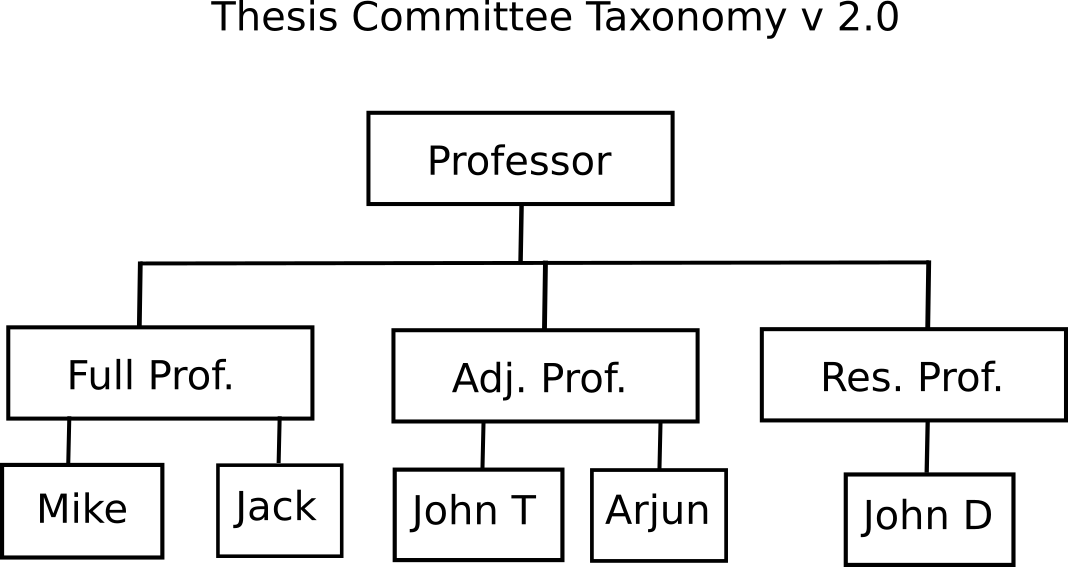
\includegraphics[width=\textwidth]{figures/tc-tax-v2.png}
\caption{Simple taxonomy of the professors and their ranks as described
in \S \ref{case-study}.}
\label{tax-1}
\end{figure}

Figure \ref{tax-2} includes the facts from all six statements. The red ``X''
marks in this figure indicate where the single relationship rule of a taxonomy
has been broken. First, in a taxonomy, all guitarists would inherit from the
same parent, or from multiple guitar-playing parents who inherit from another
guitar-playing grandparent. Second, although Mike Jr. is Mike's son
and a full professor, Mike Jr. is not a businessman and a pilot. Finally, the
relationship types between the professors, their bases classes, and the
additional occupational and familial classifications change throughout the
taxonomy in an unclear way.

\begin{figure}[htbp]
\centering
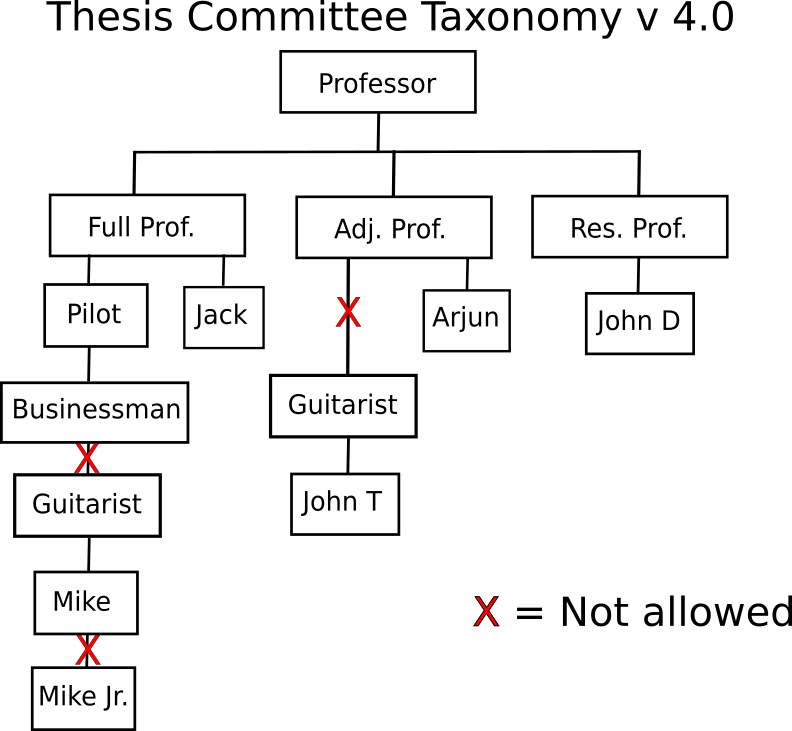
\includegraphics[width=\textwidth]{figures/tc-tax-v4-wErrors.png}
\caption{``Complete'' attempt at encoding the facts in \S \ref{case-study}.
The red ``X'' marks indicate the types of relationships that are not allowed
under the rules of a taxonomy.} 
\label{tax-2}
\end{figure}

These issues illustrate the fundamental problem with a taxonomy for
heterogeneous knowledge capture: ``Basic'' taxonomies only allow single direct
inheritance relationships to be expressed. This can be partially fixed by
allowing the relationship type to be changed based on an in-line annotation, but
what about properties such as ``can play guitar?'' Conceptually ``can play
guitar'' is not the same type of relationship as an ``is-a'' relationship. Is
a special annotation or graphic required for each new property type?
Furthermore, how does one rectify the fact that not all full professors are in
business, fly planes, or play guitar? What if a research professor did those
things as well? The complexity of the required modified taxonomy creates such a
complex diagram that one might as well simply leave the statements written
instead of encoded!

As more changes to the fundamental taxonomic data structure are required, the
required formality and bookkeeping also increase. It quickly becomes necessary
to create a separate structure simply for the purposes of managing all the
bookkeeping. Then, the data structure that uses the bookkeeping data structure
becomes something that uses the bookkeeping relationships to encode the facts.
A complex bookkeeping structure of this type that can encode classes,
relationships, and properties is an ontology, and the accompanying structure,
the graph of individuals, is known commonly as an \textit{instance graph},
\textit{knowledge graph}, or just graph of members or instances of the
ontology.

A simple ontology that describes the types of relationships, properties, and
classes for the six statements is shown in Figure \ref{ont-classes}.
Notice that this ontology contains a simple taxonomy of classes who are
Persons. Unlike the original taxonomy, Businessman, Guitarist, Pilot,
and Professor are all peers. The ontology has the following properties:
\begin{itemize}
  \item isFullProf - individuals with this property are Full Professors
  \item isAdjProf - individuals with this property are Adjunct Professors
  \item isResProf - individuals with this property are Research Professors
  \item hasSon - individuals with this property have a son whose identity is the
  object of the property
\end{itemize} 
The isFullProf, isAdjProf, and isResProf properties are all Boolean properties
that are either true or false. The \textit{hasSon} property is somewhat special
compared with the others because it encodes a relationship as a property. These
types of properties need to indicate clearly where they originate in the graph
and where they end. For statement 5 this could be indicated on the instance
graph by a property with a value of ``Mike Jr.'' or a graphic indication linking
Mike and Mike Jr.

The ontology also has the following \textit{disjoint} properties:
\begin{itemize}
  \item isFullProf != isAdjProf
  \item isFullProf != isResProf
  \item isAdjProf != isResProf
\end{itemize}
where the ``!='' indicates a negation relationship meaning ``is not.'' The
disjoint properties constrain the relationships between the normal properties
for semantic purposes. Subclasses are usually disjoint.

\begin{figure}[htbp]
\centering
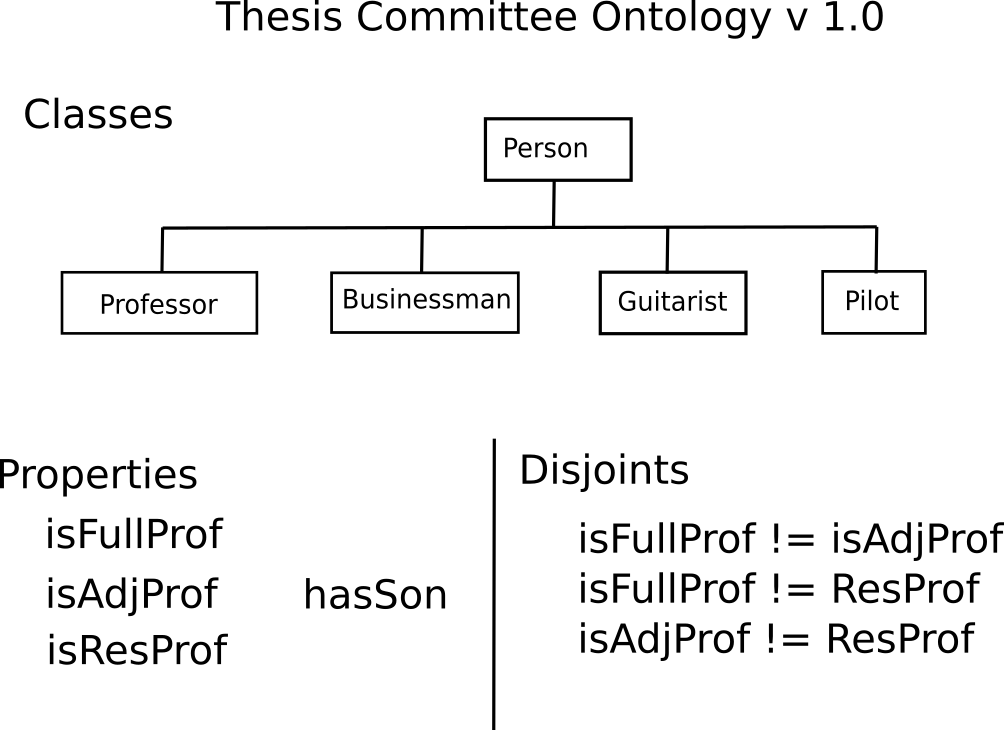
\includegraphics[width=\textwidth]{figures/tc-ont-classes.png}
\caption{Relationships, properties, and classes for the example in \S
\ref{case-study}.}
\label{ont-classes}
\end{figure}

The instance graph that uses the ontology to encode all six statements is shown
in Figure \ref{ont-instances}. This graph combines taxonomic ``is-a''
relationships and the ontological properties to fully represent the facts
and removes the representational problems found in Figure \ref{tax-2}. This
includes Mike's multiple roles and parental status. Professorial rank is
captured with properties instead of through direct inheritance. Note that the
green line in this figure has no special significance, but its color is useful
to show its path next to the black lines.

\begin{figure}[htbp]
\centering
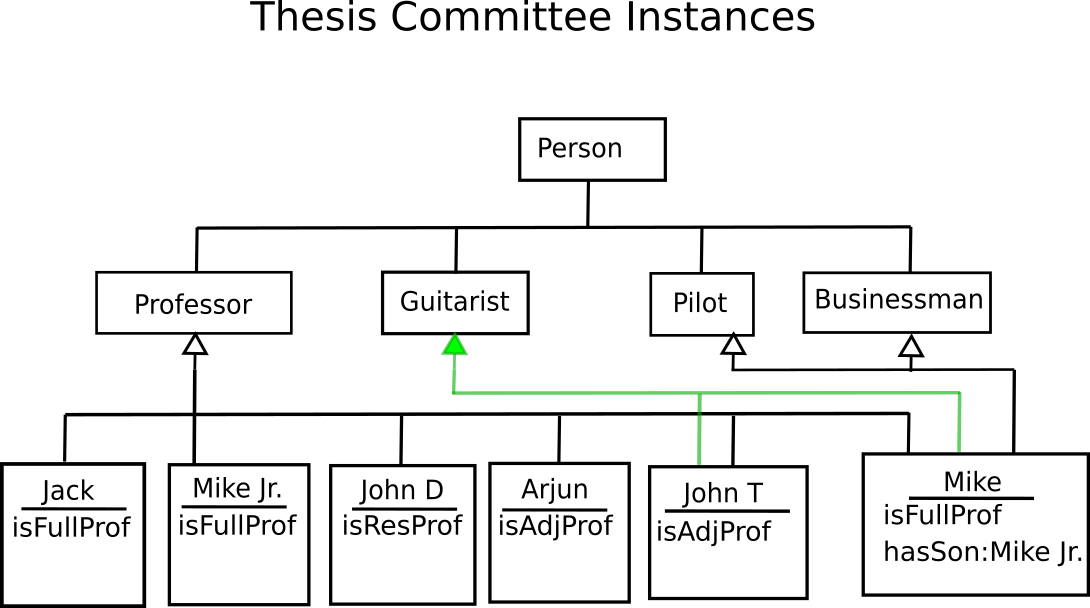
\includegraphics[width=\textwidth]{figures/tc-ont-instances.png}
\caption{Instance graph that uses the ontology in Figure \ref{ont-classes}
to encode the example in \S \ref{case-study}. The green line is not of
ontological signficnance but is colored separately to show the full connection.}
\label{ont-instances}
\end{figure}

An important aspect of ontologies, including this example, is that new facts
that are not present in the instance graph can often be inferred from the facts that
are present. Alternatively, because the graphs are open, merging graphs can
reveal new facts when inference rules are applied. Two facts that can be
inferred from the present set of facts is that an inverse relationship exists
for ``hasSon,'' which we might obviously call ``hasFather,'' and the identity of
Mike Jr.'s father is Mike. These facts are obvious to human readers, but that is
only because our experience fills in the ontological gaps. With respect to graph
mergers revealing new facts, suppose that someone merged a new ontology that
described Persons in great detail and that one property it described is that
all sons are male. It would then be possible to immediately deduce that Mike Jr.
is male.

\section{Machine-Readable Ontologies}

Real life ontologies are significantly more complex than the example in \S
\ref{case-study}. They are also used to capture and reason about large sets of
facts, which requires computational resources for processing. It is not feasible
to create any such ontology using the scheme in the example, and numerous
ontological standards have been developed. 

OWL and related languages are used for this work to
capture ontological details in a machine-readable way without sacrificing any
formality that is also useful to the human reader. OWL is based on RDFS, which
is in turn based on RDF.

Summaries of these languages are provided below based on the most recent
langauge specifications and other sources, \cite{allemang_semantic_2008}. These
summaries also include practical findings from the author who as a user of
these languages discovered a number of pitfalls that are not commonly or widely
discussed in the extant literature.

\subsection{The Resource Description Framework}

RDF is a W3C standard for exchanging data
across the internet \cite{noauthor_rdf_nodate}\cite{noauthor_rdf_nodate-3}. It
forms the basis of a so-called \textit{semantic web} where data resources are both linked and
self-describing, thus making large knowledge graphs that can be easily walked
to understand and find meaning in data.

The key concept in RDF is that statements can be made about uniquely
identifiable \textit{resources} in human and machine-readable ways. Resources
are uniquely identified with internationalized resource identifiers (IRIs) that
extend the universal resource identifier (URI) standard by adding support for
non-English characters and non-ASCII character sets. Resource names can be
anything from simple names that are locally unique to fully qualified globally
unique names.

Descriptions of resources are made with statements. Statements in RDF are
similar to sentences in the English language. Each statement contains a subject,
predicate, and object. The predicate describes the relationship of the subject
to the object in an RDF statement, just as the predicate (verb) ``is'' links the
subject ``color'' (or ``ballColor'') to the object ``red'' in ``The color of
the ball is red.'' This type of statement is called a \textit{triple}.

RDF triples are represented as full graph data structures in memory and are
serialized to any one of a number of file formats, including an XML-based format
and several formats that are easier for humans to read \cite{noauthor_resource_2019}.
Most of the supported formats for RDF are standardized, although several formats
add support for additional features not found in the standard. This includes the
JSON Linked Data (JSON-LD) and Notation3 formats. Unless otherwise
specified, the remainder of this document uses a very readable and common
serialization called the Terse RDF Triple Language (TURTL)
\cite{noauthor_rdf_nodate-4}. This format is signifcantly easier to understand
than others for humans and has the added advantage of being succinct in written
text. For example, the statement ``The color of the ball is red'' would be
rendered as a TURTLE triple with \begin{lstlisting}[language=TURTL]
<#ball>
    hasColor <red>.
\end{lstlisting}
whereas for an RDF/XML triple it would be
\begin{lstlisting}[language=XML]
<?xml version="1.0"?>
<RDF>
  <Description about="ball">
    <hasColor>red</hasColor>
  </Description>
</RDF>
\end{lstlisting}

Statements about resources can be distributed, including outside of their
current graph. In the RDF literature, this is described by the phrase ``Anyone
can say anything about anything'' (AAA). This means that for any given resource,
any other resource can be included in triples. This is akin to the ontological
openness described in \S \ref{ont-openess}. This also means that without human
intervention it is very hard to establish the origin of data for which there are
numerous distributed triples, unless one of those triples provides such a
description. Within the current graph, resource descriptions can be segmented
for clarity. If a statement such as ``Jay Jay Billings works at Oak Ridge
National Laboratory, a DOE facility,'' is made, instead of writing a single
TURTL triple that captures all the facts, it could be written as
\begin{lstlisting}[language=TURTL] <#JayJayBillings>
    worksAt <#ORNL>.
<#ORNL>
    a <#NationalLaboratory>; hasName ``Oak Ridge National
    Laboratory''^^xsd:string.,
\end{lstlisting}
which uses references to other triples and links them into the original triple
about the author.

Notice the previous listing includes the term
\begin{lstlisting}[language=TURTL]
    hasName ``Oak Ridge National Laboratory''^^xsd:string.
\end{lstlisting}
This term assigns a \textit{literal} value of ``Oak Ridge National Laboratory''
to the subject of the triple. The additional characters at the end ---
``\textasciicircum\textasciicircum xsd:string''--- set the type of the literal
to an XML schema definition string. Literal values can be set for many different types of data, including
most primitives such as integers and floating point numbers found in standard
programming languages.

Section \ref{case-study} briefly mentions the process of inference. Basic RDF
is straightforward: it describes resources. However, it is possible to include data
on the resources that establishes the relationships among them and thus makes
it possible to infer facts that are not explicitly written
\cite{allemang_semantic_2008}. This can include data shaping to conform to a
particular set of information, type restriction, or classification information.
These capabilities are provided as languages built on top of RDF, including the
RDFS and OWL.

An important aspect of RDF not covered in more detail in this work is the
ability to query it using the SPARQL query language. 

\todo{GET NOTES FROM NOTEBOOK!!!!\\}

\subsubsection{Containers}

RDF has several \textit{containers} that can hold sets of data
\cite{noauthor_rdf_nodate-3}. These include rdfs:Container, rdf:Bag, rdf:Seq,
and rdf:Alt. These containers are considered to be open, and additional data can
be added. Alternative closed containers called \textit{collections} represent
sets of data that cannot be modified and that are ordered from first to last
element. The only supported collection in the RDF specification is rdf:List.

Containers and collections are signficantly different than similarly named
structures in object-oriented programming languages, especially where generic
and templated programming is concerned.

\subsection{RDFS}

Although programming languages have preset grammars, data languages are often
left without a language that describes in machine-readable terms the allowed
values and entries in a data file. This information is provided for users in
a format specification for the data language but not in a way that can be
programmatically enforced. 

RDFS provides this capability for RDF \cite{noauthor_rdf_nodate-5}\cite{
allemang_semantic_2008}. RDFS supports describing sets of RDF resources in a
machine-readable way that can subsequently be used for validation and inference.
RDFS is itself defined in RDF, so the sets, or classes, of resources defined by
the schema are described in a standard RDF file, as are instance files
containing data that conforms to the schema.

Classes in RDFS are described by the rdfs:class descriptor in a triple. For
example,
\begin{lstlisting}[language=TURTL]
<#cat>
    rdf:type rdfs:Class;
\end{lstlisting}
defines a type of class called Cat. The rdf:type predicate is a special
statement that indicates the type of resource is specified by the
object. 

RDFS classes also support inheritance, and ``Cat'' could inherit from
``Mammal'' or ``Feline,'' as expected. The following TURTL triple illustrates
that:
\begin{lstlisting}[language=TURTL]
<#cat>
    rdfs:subClassOf <Mammal>.
\end{lstlisting}
It is also possible for properties to inherit from other properties using the
rdfs:subPropertyOf relation.

Likewise, individuals can be declared to be of a particular type. The TURTL
triple
\begin{lstlisting}[language=TURTL]
<#garfield>
    rdf:type <#cat>;
    hasName  ``Garfield''^^xsd:string.
\end{lstlisting}
describes a cat named Garfield, which we can infer to be a mammal as well.

The rdfs:subClassOf term used for inheritance is actually a property. To put
this differently, the subject of a triple with the predicate rdfs:subClassOf
has the property that it is a subclass of the other class. 

Triples are in general just maps of subjects and objects via properties.
Sometimes it is necessary to restrict what type of subject relates to a
particular type of object in this mapping. In this case, the rdfs:domain and
rdfs:range properties can be used to restrict the types of the root property.
The rdfs:domain property restricts the type of a subject, while the rdfs:range
property restricts the type of an object. It is possible to simultaneously
define rdfs:domain and rdfs:range for a property.

A select number of logic operations are supported by RDFS, including unions and
intersections. Special relations exist for the logic operations for classes and
properties alike.

Many schemas exist for reuse on the internet and are available for
public download through sites like Linked Data Applications
\cite{noauthor_linked_nodate-1}. These schemas can be included through an
approriate import call in the RDF file. In TURTL, imports are handled with the ``@prefix''
statement, as follows:
\begin{lstlisting}[language=TURTL]
@prefix rdfs: <http://www.w3.org/2000/01/rdf-schema#> .
@prefix foaf: <http://xmlns.com/foaf/0.1/> .

<#banana>
    rdf:type rdfs:Class;
    foaf:knows ``Spongebob''.,
\end{lstlisting}
where \textit{rdfs} and \textit{foaf} are imported schemas.

One nice feature of RDFS that is completely nonfunctional but useful
nonetheless is the addition of rdfs:Comment and rdfs:Label relations that make
it possible to provide detailed comments describing the data, as well as a
user-friendly label that can be substituted for default or missing data by the
display.

RDFS adds powerful features to the RDF language stack. However, as powerful as
it is, many different types of relations are missing, which restricts its
utility for more complex data relationships. Luckily, these and more are
available in OWL.

\subsection{Web Ontology Language}

OWL builds on RDF and RDFS to add additional
features for inferencing and formal ontological syntax \cite{
noauthor_owl_nodate}. The major addition to OWL over RDFS is a set of
properties that describe inverse, transitive, symmetric, and equivalent relationships
\cite{allemang_semantic_2008}. Unlike RDF and RDFS, the primary purpose of OWL
it to provide enough semantic constructs so that inferencing can be greatly
expanded for well-described data. This makes it possible for instance data that
follows an OWL ontology to be very well understood based solely on the provided
data set and the ontology.

OWL's set of default properties can be extended very easily to create new
ontological constructs by mixing the default properties in new ways. Since OWL
is serialized using RDF (which is not a strict requirement) extension is
performed simply by creating a new RDF triple that links the relevant terms.

Modeling ontologies with OWL is different than modeling in languages such as the
UML. There are many subtle differences
between the two languages, but UML is more general. In fact, OWL is
defined in part with UML models. One additional difference of particular
importance is that classes in UML can have member variables that are tied
directly to a single class. It is possible to emulate this behavior in OWL
through object properties and the rdfs:domain and rdfs:range properties that
restrict the type subject and predicate types, but without these restrictions
object properties can be used by any class. Additionally, complex members
may require pointer-like object properties linking them to their class. OWL also
allows properties to have properties, including transitive properties, which is
generally reserved only for classes in object-oriented languages.

There are several different types of OWL that can be selected based on the
preferred inference needs of the client. Since general graphs can be
computationally costly to search thoroughly, ``lighter'' versions of the
specifications with properties removed can be much faster if the data will allow
it. The complete version of OWL is commonly called OWL Full or just OWL. The two
sublanguages of OWL are OWL Lite and OWL DL. OWL Lite is a lightweight subset
of OWL on which inferencing models can be run very quickly. OWL DL
is a middle ground in terms of feature richness and performance
during inferencing \cite{noauthor_owl_nodate-2}.

\subsection{Useful Tools}

There are numerous tools, many of which are exceptional, for working with linked
data and semantic web technologies. This section provides a summary of some of
these tools, not as an endorsement but as a reference for the interested reader.

\subsubsection{Linked Open Vocabularies}

The Linked Open Vocabularies (LOV) project is a repository for ontologies from
the Ontology Engineering Group \cite{noauthor_linked_nodate-1}. The site
provides up-to-date information on ontologies and vocabularies for a large number of projects, all
of which is searchable and can be examined with a friendly web interface. This
repository can be used to find high-quality, well-tested resources instead of
writing new ones from scratch.

\subsubsection{Prot\'eg\'e}

Prot\'eg\'e is an open source ontology editor created by the Stanford Center for
Biomedical Informatics Research at the Stanford University School of Medicine
\cite{noauthor_protege_nodate}. Ontologies can be managed as individual files or
as part of version control repositories. In addition to providing general creation and
editorial support for ontologies, Prot\'eg\'e includes a large number of plugins
that provide extra tools such as visualization engines and documentation
exporters.

All of the ontologies in this work were created using Prot\'eg\'e, with only
minor edits and some initial learning work performed in different tools. This
includes the original versions of graphs shown later in the text.

\subsubsection{Apache Jena}

Apache Jena is an open source framework that supports six different projects for
semantic web and linked data applications \cite{noauthor_apache_nodate-1}. These
include an RDF utility library and SPARQL query engine, a file-based and a web-based
triple store, and ontology and inference libraries. Apache Jena is written in
Java, although the web-based triple store is available by standard HTTP calls. 
Apache Jena is very useful for writing programs that can directly manipulate
RDF resources, including storing the graphs for later use.

\subsubsection{Eclipse}

The Eclipse Platform is an open source platform that has more than 300
projects, managed by the Eclipse Foundation. The
platform includes many different tools, including a generic XML editor
that is very good for RDF/XML files and a TURTL editor, that is available as a
third-party plugin \cite{ noauthor_xturtle_nodate}. The platform includes
additional tools for managing basic file manipulation for ontologies and RDF
data. It also includes tools for managing software and data repositories. The
majority of this dissertation was written using the Texlipse plugin to Eclipse.

\subsubsection{Graphviz}

Graphviz is a powerful graph visualization tool that supports the Dot language
\cite{noauthor_graphviz_nodate}. Nodes in graphs are drawn as circles with
labels and connections between the nodes are drawn as curves with annotations
that describe their connection type. This is very useful for RDF graphs where
both the node types and connections vary depending on the details of the triple.

\subsection{Our Case Study in RDF and OWL}

\begin{figure}[htbp]
\centering
\baseIncludegraphics{exampleOntology/exampleOntology.png}
\caption{Graphviz plot of the combined thesis committee ontology and its
individuals.}
\label{example-ont-graphic}
\end{figure}

The previous sections provide all that is needed to create a simple,
formal, machine-readable ontology for the thesis committee example at the
beginning of this chapter. As a pedagogical tool, that example is fine, but as
an example of a real ontology it suffers from being written by just another guy
in his arm chair! Using the tools of the previous section, it can be turned
into something very similar to what will be developed for scientific workflows,
as well as ontologies commonly available in the LOV
repository. Figure \ref{example-ont-graphic} shows the committee ontology and
its individuals rendered in a single Graphviz graph. Listing
\ref{example-ont-listing} shows the same content as the graph but in its
formal TURTL serialization.

\lstinputlisting[language=TURTL,caption=The complete OWL ontology
for the example problem.,label=example-ont-listing]{/home/bkj/thesis/exampleOntology/exampleOntology.turtl.owl}

The ontology and its individuals were created completely in Prot\'eg\'e using an
in-memory representation of the graph. Exports were created for both the
Graphviz plot and the TURTL file. Apache Jena can readily consume the TURTL file
for further processing.

\section{Summary}

This chapter introduces the concept of an ontology, including its common
features and the fundamental differences between ontologies and taxonomies. A
simple example is presented that shows how even simple relationships can be
difficult to capture without the formalism and reasoning abilities of
ontological tools.

The RDF-based languages for working with RDF, RDFS, and OWL are described with
a particular focus on those features that are most useful to this work. Useful
tools for creating ontologies and RDF models are also presented.

Finally, the original committee example was revisited using the tools and
techniques described for the RDF-based languages. This introduces formality,
structure, and machine-readable properties that put the example, as simple as it
is, on par with ontologies of much broader appeal.

Using the languages and tools presented in this chapter, and the description of
scientific workflows and workflow engines provided elsewhere in this work, it is
now possible to pursue the goal of creating an ontology that accurately
describes the phantasmagoria of scientific workflows.

    \chapter{Scientific Workflow Ontology}
\label{ch:workflow-ontology}

The tools, techniques, and background knowledge provided in the previous
chapters makes it possible to answer important questions about an eclectic mix
of workflow technologies. These questions include ``What is a workflow?'' and
``Are workflow management systems conceptually the same?,'' ---all with the goal
of establishing whether the tools are varied or merely variegated. The first of
these two questions ---``What is a workflow?''--- is of particular interest in
this work because a better understanding of the different types of workflows will
present the opportunity to examine problems that were previously too costly in
manual labor or altogether impossible.

The following sections present a workflow ontology, \S
\ref{workflow-ont-section}, and the method used to develop it, \S
\ref{workflow-ont-method}. Finally, concrete examples of the application of this
ontology to workflows ```in the wild'' are provided to show its range as a
decision-making and scientific computing tool.

\section{Methodology}
\label{workflow-ont-method}

\todo{Talk about design philosophy?}

The scientific workflow ontology presented in \S \ref{workflow-ont-section} was
developed by considering workflows in two environments: i) the context
of problems they solve and ii) as entities that are executed by workflow
management systems.

\subsection{Workflow Problems}

Workflows are most interesting in the context of problems they solve. As
Chapter \ref{ch:introduction} demonstrates, because of the large number of these
problems, it can be very difficult to write an all-encompassing
definition of a scientific workflow by looking only at the workflows directly. 

One classic way to solve calculus problems without an obvious solution is the
method of change of variables in which new variables related to the original
variables by some relationship are used in place of the originals. Changing
variables makes it possible to mask certain types of complexity to reveal direct
methods of solving the problem. An analogy to this method can be used to study
scientific workflows. Specifically, seeking a definition for workflow problems
instead of workflows can make it possible to find a definition of scientific
workflows by ``solving'' for it. 

It is sufficient for the purpose of this work to define a workflow problem
by building an ontological model based on the description of workflow
management systems, workflows, and data in other chapters. Workflow problems of
any of type can be decomposed into three required components: i) The workflow
description, ii) the workflow engine or management system that executes the
workflow based on the description, and iii) the data required to fully describe
and execute the workflow. The latter may include ---but does not necessarily
require--- metadata that describes the contents of the data itself, bulk data
including values and quantities of interest used in the workflow. (For the purposes of
this work, it is sufficient to consider provenance information as a type of
metadata.) A workflow problem, then, is one that is solved by providing a
workflow description to a workflow management system with all pertinent data in
hand. Thus, by examining the set of workflow problems and workflow management
systems, while allowing data to act as a kind of free variable, it is possible
to describe the set of workflows completely.

This is an empirical way of thinking about workflows that results in an emergent
definition, versus a prescribed one. This method accepts the community will
move as it sees fit, but asserts (quite strongly) that progress can still be
made by considering what exists collectively. The method is additive since
any new workflow management system can be studied to learn about the
workflows it supports, and the description of those workflows can be added to
the model created by the original effort. As the model grows, it will enclose a
larger area of the workflow space, resulting in the emergence of a new or
updated description of the set of abstract workflows.

This method responds well to a modeling treatment, and, indeed, may be described
as a modeling method. All the languages and tools in Chapter \ref{ch:ontologies}
can be applied.

\subsection{Referenced Workflow Management Systems}

Workflows from several workflow management systems were examined as part of this
work. This include workflows from Eclipse ICE, Taverna
\cite{wolstencroft_taverna_2013}, Triquetrum \cite{brooks_introducing_2016},
Pegasus \cite{noauthor_pegasus_nodate}, the Common Workflow Language
\cite{noauthor_common-workflow-language:_2018}, Cylc
\cite{noauthor_cylc_nodate}, Chiron \cite{ ogasawara_chiron:_nodate}, Moteur
\cite{glatard_flexible_2008}, and SAW \cite{clay_incorporating_2015}. One
unnamed heirarchical workflow management system from Argonne National
Laboratory was also reviewed.

\section{Workflow Ontology}
\label{workflow-ont-section}

This section describes an ontology for scientific workflows created using the
method and philosophy described in the previous section. Classes, object
properties, and data properties are listed subsequently. The full OWL ontology,
(created in Prot\'eg\'e), is provided as a TURTL file in Appendix
\ref{app:full-ontology} to preserve space for the narrative here. The full
TURTL file includes some axioms not discussed here. 

Unlike the example in Chapter \ref{ch:ontologies}, no individuals are described
in this section. The following figures are Graphviz visualizations
of subgraphs of the main ontology graph pulled from Prot\'eg\'e using its OntoGraf
plugin. These figures illustrate the relationships among the core classes and
properties of the ontology. Table \ref{ont-stats-table} summarizes numerous
metrics of the ontology.

\begin{table}[H]
\begin{tabularx}{\textwidth}{|X|X|}
\hline
Triple count & 241 \tabularnewline\hline
Axiom count	& 161	\tabularnewline\hline
Logical axiom count	& 53	\tabularnewline\hline
Declaration axioms count &	40	\tabularnewline\hline
Class count	& 25	\tabularnewline\hline
Object property count	& 9	\tabularnewline\hline
Data property count	& 3	\tabularnewline\hline
Individual count &	0	\tabularnewline\hline
Annotation property count	& 8 \tabularnewline\hline
SubClassOf	& 21		\tabularnewline\hline
DisjointClasses  &	5 \tabularnewline\hline
SubObjectPropertyOf	& 3 \tabularnewline\hline
ObjectPropertyDomain &	10	\tabularnewline\hline
ObjectPropertyRange	& 7 \tabularnewline\hline
SubDataPropertyOf	& 1 \tabularnewline\hline
DataPropertyDomain	& 4	\tabularnewline\hline
DataPropertyRange &	2 \tabularnewline\hline
AnnotationAssertion	& 68 \tabularnewline\hline
\end{tabularx}
\caption{Ontology Statistics}
\label{ont-stats-table}
\end{table}

The full ontology is also preserved in the Eclipse ICE GitHub repository
\cite{billings_ice_2019}.

%%% Include generated ontology text.
\baseInclude{chapters/ice-workflows.out.tex}

\section{Examples and Applications}
\label{workflow-ont-examples}

This section shows examples and applications of workflows marked up as
instances of the workflow ontology. The full RDF listings for all
examples are provided in the appendices.

\subsection{Basic File Move}
\label{move-workflow}

The first example is a very simple workflow showing the move of a file from
one location to another. The workflow description executes a single task, which
is specialized to move a file using a dedicated action type. The action type
uses a Java class as its target, and it uses simple string values for file name
input and output.

This example is important because it shows how simple it is to wire together a
straightforward workflow. The relationships among workflow descriptions,
tasks, and actions create a directed acyclic graph for this type of workflow.
However, it is also important because file transfer is a common task in many
workflows, often occurring as a subworkflow that executes before and after
other tasks or before and after the main workflow.

Figure \ref{move-workflows} shows a version of this example that has been
slightly edited to better fit the page. The full TURTL version of this workflow
is available in the appendices, \S \ref{app:move-workflow}.

\begin{figure}[htbp]
\centering
\baseIncludegraphics{figures/moveWorkflow.png}
\caption{The basic file move workflow.}
\label{move-workflows}
\end{figure}

\subsection{Combining Cycles and Loops}

The next example covers a more complicated use case that is arguably uncommon
in more popular workflow engines: cycles and loops. This example, depicted in
figure \ref{cycle-loop-test}, describes a simple workflow were 50 files are
created using a threshold limiter and then deleted through a standard
50 iteration loop. A threshold limiter limits the amount of something --- in
this case the number of files created --- based on a threshold.

This workflow is a simple model, but it is a good analog to more complicated
systems in which data is gathered until a threshold is crossed, such as
the number of counts from a detector, and then the set of files are processed in a loop. A
threshold is well modeled by a cycle because the system waits until the
threshold is met, which requires a periodic (cyclic) check against the limit.

The examples contains two tasks, \#loopTask and \#cycleTask, with the \#loopTask
being dependent on \#cycleTask. The dependency is because \#cycleTask
creates the files, which must all exist before the \#loopTask is executed. The
action of the cycle task is to create a file using the Linux ``touch'' command,
and its condition is to created files until the number of files in the directory
is greater than 50. It checks the number of files using a Java program called
``fileCounter.'' When this task is complete, the dependency for \#loopTask is
satisfied and it can execute its action --- the Linux ``rm'' command to remove a
file. The condition on the loop is that its action is executed for fifty
iterations specified by the lowerBound, upperBound, and stepSize properties.

Workflows such as this are easy to model in workflow systems where loops and
cycles are supported. It is also possible to execute this workflow in systems
that do not directly support those constructs by decomposing it into smaller
workflows since the number of files is fixed. The \#cycleTask can be
executed as a linear graph of fifty separate system checks. The \#loopTask can
be unrolled to fifty separate executions of the remove command. However, limited
polling and unrolling, respectively, only work in cases where the total number
of iterations is fixed.

\begin{figure}[htbp]
\centering
\baseIncludegraphics{figures/cycle-loop-test.png}
\caption{Combined cycle and loop workflow example.}
\label{cycle-loop-test}
\end{figure}

The full TURTL version of this workflow is available in the appendices, \S
\ref{app:cycle-loop-test}.

\subsection{Pegasus Split Example}

The Pegasus workflow management system is especially good at executing large,
parallel workflows. The Pegasus website and documentation provide a simple
example of splitting files into parts in parallel
\cite{noauthor_workflow_nodate}. The workflow model of Pegasus is very well
paired with the workflow ontology, and mapping this example from its source can
be accomplished in a very straightforward fashion.

Figure \ref{pegasus-split-workflow} is graph of the Pegasus splitting example
showing only the most essential parts, namely, tasks, actions, action types, and
properties from the workflow ontology. Files and parameters in Pegasus map
directly to properties in the ontology, with the jobs that are executed against
them mapping to tasks and actions. This example illustrates how quickly even a
simple workflow can become too hard to easily visualize in its entire scope, so
figure \ref{pegasus-comparison} shows i) a greatly slimmed down version of the
worfklow graph that contains only the tasks compared against ii) the original
graph of the image from the Pegasus website.

One important difference of the workflow ontology that is highlighted by
Figure \ref{pegasus-comparison} is that it models workflow tasks and their
dependencies, whereas other workflow models are focused on data flow. This is
highlighted by the inversion of the arrow heads across the sides of the image.
In part a), the arrows point from the tasks at the top of the dependency chain
down to the initial task that has no dependencies against it. The opposite is
true in part b), which shows the initial task with no dependencies generating
output that is fed into the tasks where it is required. 

Both views are correct: They are equally valid perspectives are akin
to saying that ``The donkey pulls the cart'' and ``The cart is pulled by the
donkey.'' As long as the interpreter gets the point that the cart needs to move,
there is not problem. This inverted graph phenomenon is also witnessed in
provenance graphs when compared against workflows they describe (see \S
\ref{provenance-background}).

\begin{figure}[htbp]
\centering
\baseIncludegraphics{figures/pegasusSplit.png}
\caption{Only the most essential elements of the Pegasus split
example as marked up in the workflow ontology. This level of detail ---far
removed from the full details--- shows the high number of facts captured with
semantic models.}
\label{pegasus-split-workflow}
\end{figure}

\begin{figure}[htbp]
\centering
\baseIncludegraphics{figures/pegasus-comparison.png}
\caption{Graph of Figure \ref{pegasus-split-workflow} on the left with only
the tasks shown compared with the original Pegasus split example from the
website on the right.}
\label{pegasus-comparison}
\end{figure}

The full TURTL version of this workflow is available in the appendices, \S
\ref{app:pegasus-workflow}.

\subsection{Eclipse ICE II/III Task Model}

Eclipse ICE, covered extensively in Chapter \ref{ch:eclipse-ice},
uses a somewhat unique view of workflows in its workflow model. Workflows
in Eclipse ICE are executed as finite state machines that can include human
feedback, conditional branching, and error conditions. This makes it possible
to describe workflows in a conceptually abstract way using state machine
theory. It remains possible to model the execution flow of these state machines
as directed acyclic graphs, which can be observed in Figure \ref{ice-workflow}.
When cast into the workflow ontology, it is clear that the abstract workflow
executed by ICE is directed and acyclic, even if its instances may execute with
cycles and other conditions.

ICE workflows start by setting up the Form used to collect
\#workflowProperties, which is the \#setupFormTask. The workflow continues
through multiple tasks that depend on the initial Form, as well as other tasks,
and which cause state changes within the system. On state changes, the task
executes the \#stateChangeAction to update the system state, reconfigure data,
and prepare the next task. User feedback is required, and the \#submitForm task
will wait until this condition is met before transitioning to review and
processing. Like the earlier examples, arrows point from tasks to previously
executed tasks through the ``dependsOn'' property such that the last task,
\#processTask, shows up at the top and does not appear to feed any other tasks.

The system goes from one task to another through the state changes. Each state
change configures the system so it can execute its next task and ensures
that all previous steps were executed properly. Thus, the internal logic of when
a task is complete remains internal to the workflow, and no external logic is
required to satisfy task completion.

This example shows a very interesting relationship between the \#hasCondition
and \#dependsOn object properties in the ontology: Conditions are merely
special, internal dependencies that are managed directly by the task instead of the
workflow engine. Conditions execute small ``micro-workflows'' within the task
that affect its completion, while the workflow engine manages its completion by
first executing the tasks on which it depends. Thus, conditions can be thought
of as merely subgraphs of the larger workflow that sit between a task and its
dependencies.

\begin{figure}[htbp]
\centering
\baseIncludegraphics{figures/iceWorkflow.png}
\caption{The tasks, actions, and states of the standard workflow model of
Eclipse ICE, as graphed using the workflow ontology.}
\label{ice-workflow}
\end{figure}

The full TURTL version of this workflow is available in the appendices, \S
\ref{app:ice-workflow}.

\subsection{Neutron Scattering User Workflow and Data Pipeline}

The Spallation Neutron Source and the High-Flux Isotope Reactor operated by Oak
Ridge National Laboratory are the premiere neutron sources in the United States.
Figure \ref{neutron-workflow} shows the idealized, conceptual workflow that
users can expect while performing experiments at the
facility.\footnote{Image and information courtesy of the author.} This is a good
example of the conceptual workflows mentioned in Chapter \ref{ch:introduction},
\S \ref{workflows}, because it cannot be executed and represents high-level,
idealized tasks.

\begin{figure}[htbp]
\centering
\baseIncludegraphics{figures/neutronWorkflow.png}
\caption{Conceptual neutron scattering user workflow and data pipeline.}
\label{neutron-workflow}
\end{figure}

Figure \ref{neutron-workflow-graph} shows the graph of this workflow when
translated to the workflow ontology. One immediate observation is that
conceptual workflows may not require a deep translation to be understandable
and that in some cases only tasks are needed to describe conceptual workflows.
Still, it is useful to look at conceptual worfklows in the same framework as
concrete workflows to understand how conceptual workflows can evolve to be
concrete and executable in the future.

Another important observation is that this workflow is cyclic. It is tempting to
believe that the Design of Experiments task is the first task because it is the
top-most, left-most task in the diagram, which to English speakers may suggest
that it is special. It is true that in some cases Design of Experiments may be
the first task, but many users walking through this workflow start at other
points, such as ``HPC, Modeling/Simulation, AI/ML'' because they approach
the problem from a theoretical perspective. There are several others cycles
between the various parts of the graph, such as the ``Data Reduction'' to
``Data Curation and Archival'' to ``HPC, Modeling/Simulation, AI/ML'' cycle.

\begin{figure}[htbp]
\centering
\baseIncludegraphics{figures/neutronWorkflow-graph.png}
\caption{Conceptual neutron scattering user workflow and data pipeline
graphed in the workflow ontology.}
\label{neutron-workflow-graph}
\end{figure}

The full TURTL version of this workflow is available in the appendices, \S
\ref{app:neutron-workflow}.

\section{Summary}
\label{workflows-ont-summary}

This chapter presents the methodology and reasoning behind creating a workflow
ontology using the methods discussed in Chapter \ref{ch:ontologies}, the
ontology for scientific workflows itself, and five examples of scientific
workflows mapped or translated into instance graphs of the ontology. The
examples, in particular, demonstrate the central thesis of this work that a
comprehensive metamodel of scientific workflows could describe multiple types of
scientific workflows. This includes high-throughput (Pegasus); modeling and
simulation (Eclipse ICE); iterative workflows that run repeated, looping, and
cyclic tasks (the cyclic looping example); and purely conceptual workflows that
are not executed by machines; but remain important for communication and other
work (neutron scattering user workflow and data pipeline). The examples
further demonstrate that common patterns can be described by the ontology
in a common way that is agnostic to the underlying platform, much like
design patterns in programming (Move Workflow example). 

What remains is the final question of this thesis: If scientific workflows can
be uniformly described, what are the implications for interoperability? Chapter
\ref{ch:interoperability} will seek to address this question by examining the
many different facets of interoperability.

    \chapter{Ontological Interoperability} \label{ch:interoperability}

Discuss wrapping workflow engines instead of native execution
    \chapter{Workflows on the Blockchain} \label{ch:blockchain}

Important realization with data in an open world is how do you manage it? Actors
must be free to\ldots
*Describe what they have
*Store bulk data
*Share what they have

This chapter describes a system that was developed as part of this thesis work
to address these concerns for ICE III.

\baseInclude{pubs/billings-workflows-blockchain/content}
    \chapter{Conclusions}\label{ch:conclusions}

Epistomological
POINT 1 from about next-generational problems, etc.

NOTE change in strategy from CBB, also Kingmakers and Building Microservices.

\baseInclude{pubs/workflows-paper/src/discussion}

\listoftodos
    %%%%%%%%%%%%%%%%%%%%%%%%%%%%%%%%%%%%%%%%%%%%%%%%%%%%%%%%%%%%%%%%%%%%%%%%%%%%%%%%%%%%%%%%%%%%%%%%%%%%%
    % BIBLIOGRAPHY
    %%%%%%%%%%%%%%%%%%%%%%%%%%%%%%%%%%%%%%%%%%%%%%%%%%%%%%%%%%%%%%%%%%%%%%%%%%%%%%%%%%%%%%%%%%%%%%%%%%%%%
    \makeBibliographyPage % make the bibliography title page
\newpage

% To make the bibliography, use \utbiblio{#1}{}{} command. Always use "#1" for
% the first entry. The second entry is your bibliography style, and the third
% entry is the name of your bibliography file (.bib file extension)
% bibliography style - recommend using apalike-doi as it hyperlinks DOIs Be
% sure to run BibTeX in order to generate the bibliography correctly.

\utbiblio{#1}{apalike}{bib}

    %%%%%%%%%%%%%%%%%%%%%%%%%%%%%%%%%%%%%%%%%%%%%%%%%%%%%%%%%%%%%%%%%%%%%%%%%%%%%%%%%%%%%%%%%%%%%%%%%%%%%
    % APPENDIX - OPTIONAL - COMMENT OUT IF NOT NEEDED
    %%%%%%%%%%%%%%%%%%%%%%%%%%%%%%%%%%%%%%%%%%%%%%%%%%%%%%%%%%%%%%%%%%%%%%%%%%%%%%%%%%%%%%%%%%%%%%%%%%%%%
    
    \makeAppendixPage{2}   % Input the number of appendices
    \appendix    
    \chapter*{Full Workflow Ontology}
\label{app:full-ontology}

\section{Workflow Ontology Specification}

\lstinputlisting[language=TURTL,caption=The complete
scientific workflow ontology,
label=workflow-ont-listing]{/home/bkj/thesis/xslt/ice-workflows.turtl}

%    
\section{Summary of Stuff}
some text here
\subsection{More Things}
some equations here

\subsection{Other Aspects}
some equations also here
    %%%%%%%%%%%%%%%%%%%%%%%%%%%%%%%%%%%%%%%%%%%%%%%%%%%%%%%%%%%%%%%%%%%%%%%%%%%%%%%%%%%%%%%%%%%%%%%%%%%%%
    % A VITA IS REQUIRED
    %%%%%%%%%%%%%%%%%%%%%%%%%%%%%%%%%%%%%%%%%%%%%%%%%%%%%%%%%%%%%%%%%%%%%%%%%%%%%%%%%%%%%%%%%%%%%%%%%%%%%
    \addToTOC{Vita}
    \chapter*{Vita} \label{ch:vita}

Jay Jay Billings is a Research Scientist in the Neutron Scattering
Division (NSD) and Computer Science and Mathematics Division (CSMD) at Oak Ridge
National Laboratory. He leads the Scientific Computing and Software Engineering group
in NSD and Research Software Engineering group in CSMD. He holds the Bachelor’s
Degree in Physics from Virginia Tech, class of 2005, and the Master of Science
in Theoretical Astrophysics from the University of Tennessee, class of 2008.
Mr. Billings’ research focuses on the design and implementation of modeling and
simulation tools for energy science, a large part of which has been related to
the study of scientific workflows in an HPC context.

At Oak Ridge National Laboratory, Mr. Billings is leading the Scientific
Software Initiative within CSMD and is a member of the Software Council, both of
which are taking a new look at the way ORNL develops software for the Department of
Energy. He is a founding member and current chair of the Science Working Group
at the Eclipse Foundation, where he also leads the Eclipse Integrated
Computational Environment and the Eclipse Advanced Visualization Project. Mr.
Billings was also appointed to the Eclipse Architecture Council in 2016, and is
a mentor for several additional Eclipse projects. He is a member of the
Association for Computing Machinery.

Mr. Billings has been funded by the Department of Energy Offices of Nuclear
Energy, Energy Efficiency and Renewable Energy, Advanced Scientific Computing
Research, Basic Energy Sciences, and Advanced Manufacturing.

In addition to his day job, Mr. Billings is a candidate for the PhD in Energy
Science from the Bredesen Center for Interdisciplinary Research and Education at
the University of Tennessee. He spends his spare time with his family, and
singing.

\end{document}
